\begin{figure}[htb]
	\begin{center}
		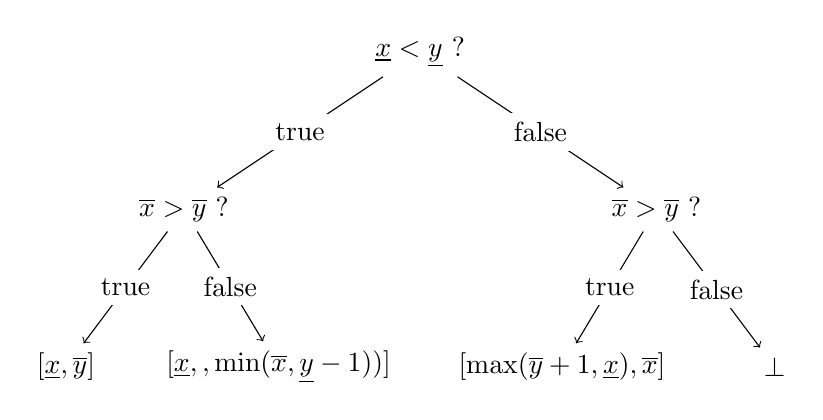
\begin{tikzpicture}
         
         \node [rectangle] (A)  at (0,0)    {$\underline{x}<\underline{y}$ ?};
         \node [rectangle] (B)  at (3,-2)    {$\overline{x}>\overline{y}$ ?};
         \node [rectangle] (C)  at (-3,-2)    {$\overline{x}>\overline{y}$ ?};
         \node [rectangle] (D)  at (4.5,-4)    {$\bot$};
         \node [rectangle] (E)  at (1.8,-4)    {$[\max(\overline{y}+1, \underline{x}), \overline{x}]$};
         \node [rectangle] (F)  at (-1.8,-4)    {$[\underline{x},,\min(\overline{x},\underline{y}-1))]$};
         \node [rectangle] (G)  at (-4.5,-4)    {$[\underline{x},\overline{y}]$};

  		 \draw [->] (A) -- node[fill=white!5]{false} (B) ;
  		 \draw [->] (A) -- node[fill=white!5]{true} (C) ;
  		 \draw [->] (B) -- node[fill=white!5]{false} (D) ;
  		 \draw [->] (B) -- node[fill=white!5]{true} (E) ;
  		 \draw [->] (C) -- node[fill=white!5]{false} (F) ;
  		 \draw [->] (C) -- node[fill=white!5]{true} (G) ;
         
        \end{tikzpicture}
        \caption{A decision diagram showing how to determine the restriction ``not equal to $[\underline{y},\overline{y}]$'' for an interval value of $[\underline{x},\overline{x}]$.}\label{fig:unequal_restriction}
	\end{center}
\end{figure}